\documentclass[11pt,a4paper,oneside]{scrartcl}

\usepackage[utf8]{inputenc}
\usepackage[ngerman]{babel}
\usepackage{amsmath, amssymb, amsthm} 
\usepackage{graphicx, tikz} 
\usepackage{hyperref} 

\newtheorem{satz}{Satz}[section]
\newtheorem{lemma}[satz]{Lemma}
\newtheorem{proposition}[satz]{Proposition}
\newtheorem{definition}[satz]{Definition}
\newtheorem{bemerkung}[satz]{Bemerkung}

\begin{document}

\title{Ausarbeitung zum Thema [XY]}
\subtitle{Bachelor-Seminar "`Top 10 Algorithms in Data Mining"'}



\author{Marcel} 
\date{\today} 

\maketitle

\tableofcontents


\begin{abstract}
\noindent\textbf{Abstract:} 
Fassen Sie hier den Inhalt ihrer Ausarbeitung kurz zusammen.
\end{abstract}

\section{Erster Beispielabschnitt}
Hallo. Ich bin ein kleiner Blindtext. Und zwar schon so lange ich denken kann. Es war nicht leicht zu verstehen, was es bedeutet, ein blinder Text zu sein: Man ergibt keinen Sinn. Wirklich keinen Sinn. Man wird zusammenhangslos eingeschoben und rumgedreht – und oftmals gar nicht erst gelesen. Aber bin ich allein deshalb ein schlechterer Text als andere? Na gut, ich werde nie in den Bestsellerlisten stehen. Aber andere Texte schaffen das auch nicht. Und darum stört es mich nicht besonders blind zu sein. Und sollten Sie diese Zeilen noch immer lesen, so habe ich als kleiner Blindtext etwas geschafft, wovon all die richtigen und wichtigen Texte meist nur träumen.

Neben diesem wundervollen Blindtext enthält dieser Abschnitt außerdem auch noch einen bekannten mathematischen Satz.

\begin{satz}[Satz des Pythagoras]\label{satz:beispiel}
Seien $a$ und $b$ die Längen der Katheten und $c$ die Länge der Hypotenuse eines rechtwinkligen Dreiecks. Dann gilt
\[
a^2 + b^2 = c^2.
\]
\end{satz}
\begin{proof}
Hier könnte ein Beweis stehen, allerdings kennt den vermutlich eh jeder.
\end{proof}

\section{Noch ein Beispielabschnitt}
Hier gibt es nichts zu sehen. Außer natürlich die wundervolle Grafik in Abbildung~\ref{fig:beispielabbildung}. Diese wurde mit dem folgenden Code erzeugt:
\begin{verbatim}
\begin{figure}
\centering
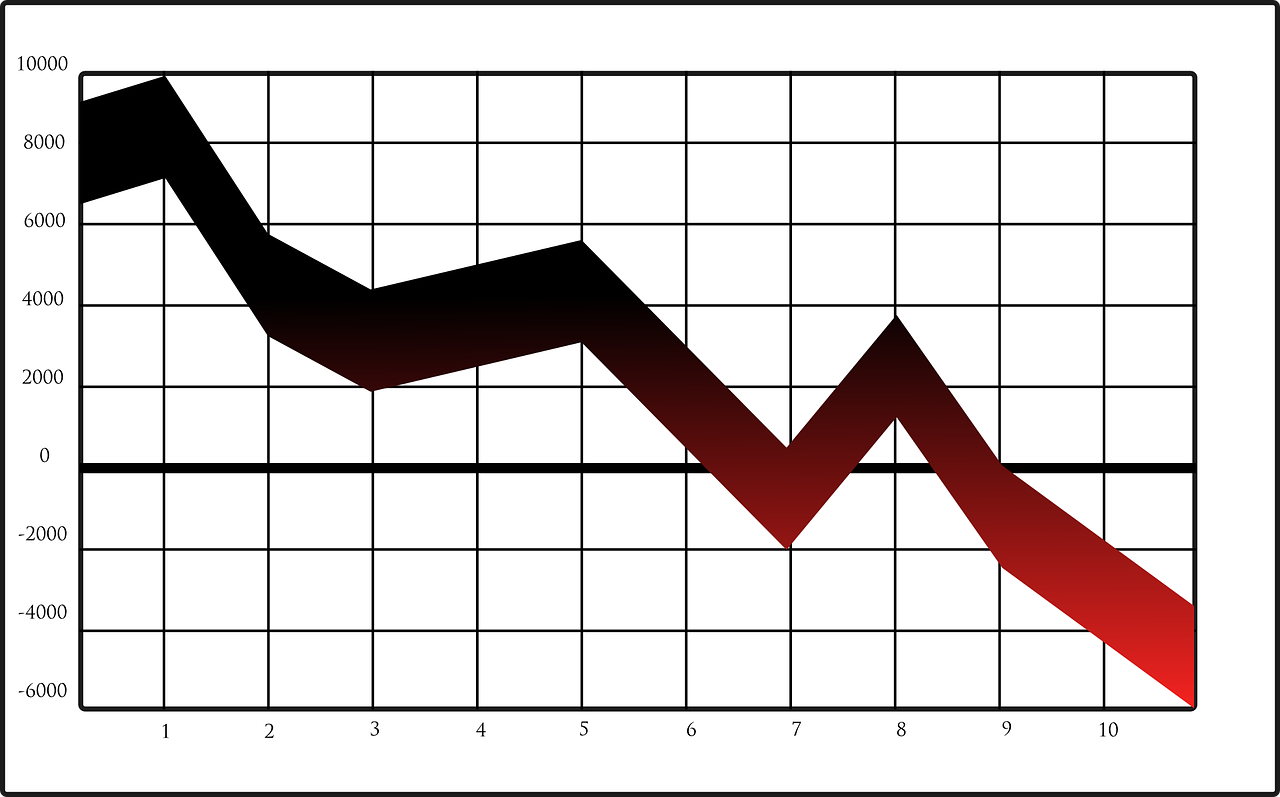
\includegraphics[width=.5\textwidth]{figures/beispielgrafik}
\caption{Dies ist ein Beispieldiagramm. Niemand weiß so genau, 
was hier eigentlich dargestellt ist\dots}\label{fig:beispielabbildung}
\end{figure}
\end{verbatim}

\begin{figure}
\centering
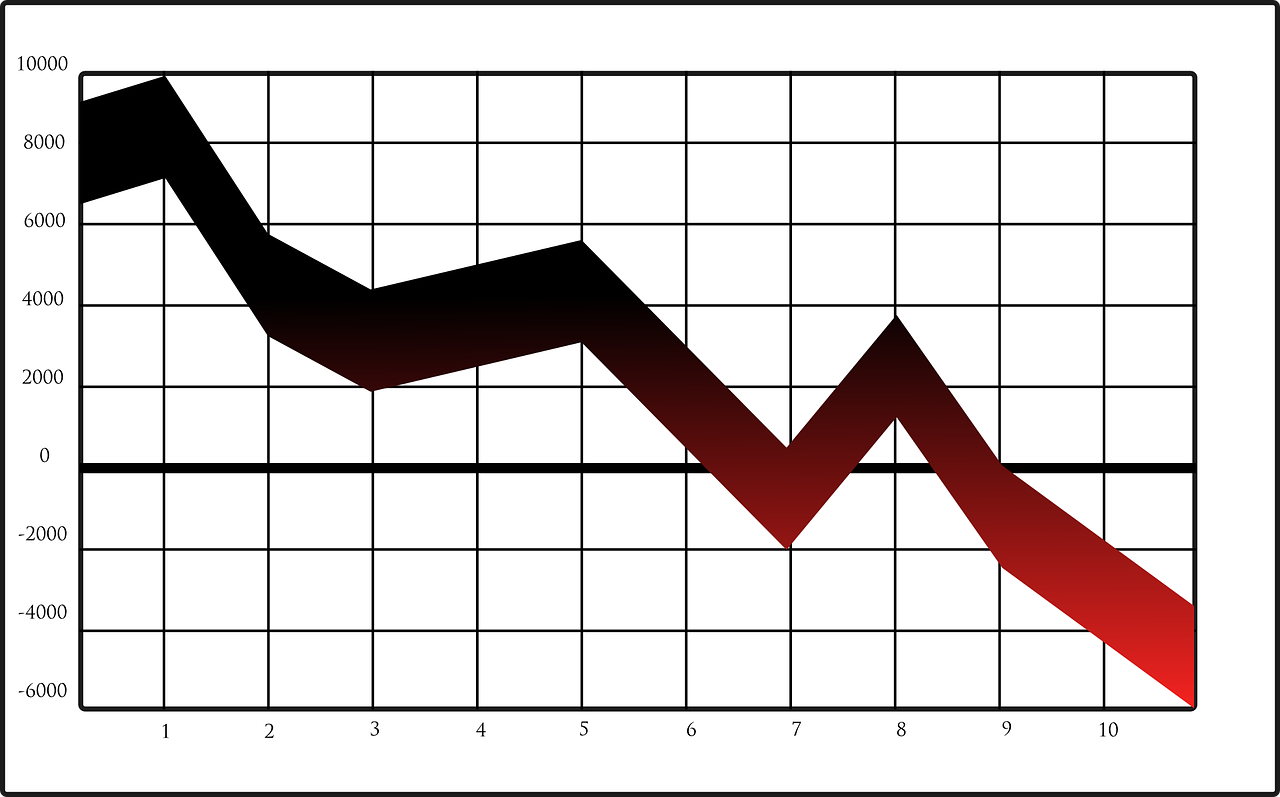
\includegraphics[width=.65\textwidth]{figures/beispielgrafik}
\caption{Dies ist ein Beispieldiagramm. Niemand weiß so genau, was hier eigentlich dargestellt ist\dots}\label{fig:beispielabbildung}
\end{figure}

\section{Einfügen von Literaturverweisen}

Am einfachsten lässt sich das Literaturverzeichnis mittels \texttt{bibtex} verwalten. Dazu liegt bereits die Datei
\texttt{seminar\_top10.bib} bei, welcher zunächst nur den einen Bibliographie-Eintrag für das dem Seminar zu Grunde liegende Buch enthält. Sie können beliebige weitere Literatur hinzufügen, die Sie verwendet haben.

Auf die in \texttt{seminar\_top10.bib} vorhandenen Bibliographie-Einträge können Sie dann mittels des \verb|\cite{}|-Kommandos verweisen. Beispielsweise erzeugt
\begin{verbatim}
Alle Vorträge des Seminars basierten auf dem Buch~\cite{WuKumar2009}.
\end{verbatim}
die folgende Ausgabe:
"`Alle Vorträge des Seminars basierten auf dem Buch~\cite{WuKumar2009}."'

\bibliographystyle{alpha}
\bibliography{seminar_top10.bib}

\end{document}
